\chapter{Study Two Documentation \label{cha:app6}}

This appendix provides documentation related to Study Two of the evaluation
stage described in Chapter \ref{cha:evaluation}. The documents included in this
appendix are:

\begin{itemize}
  \item Invitation poster for students to participate in the experiment.
  \item Study protocol followed by each group.
  \item Background and Exit questionnaire for the participants.
  \item Screenshots of the concept maps created by the participants during the
  experiment.
  \item Exit questionnaire responses.
\end{itemize}

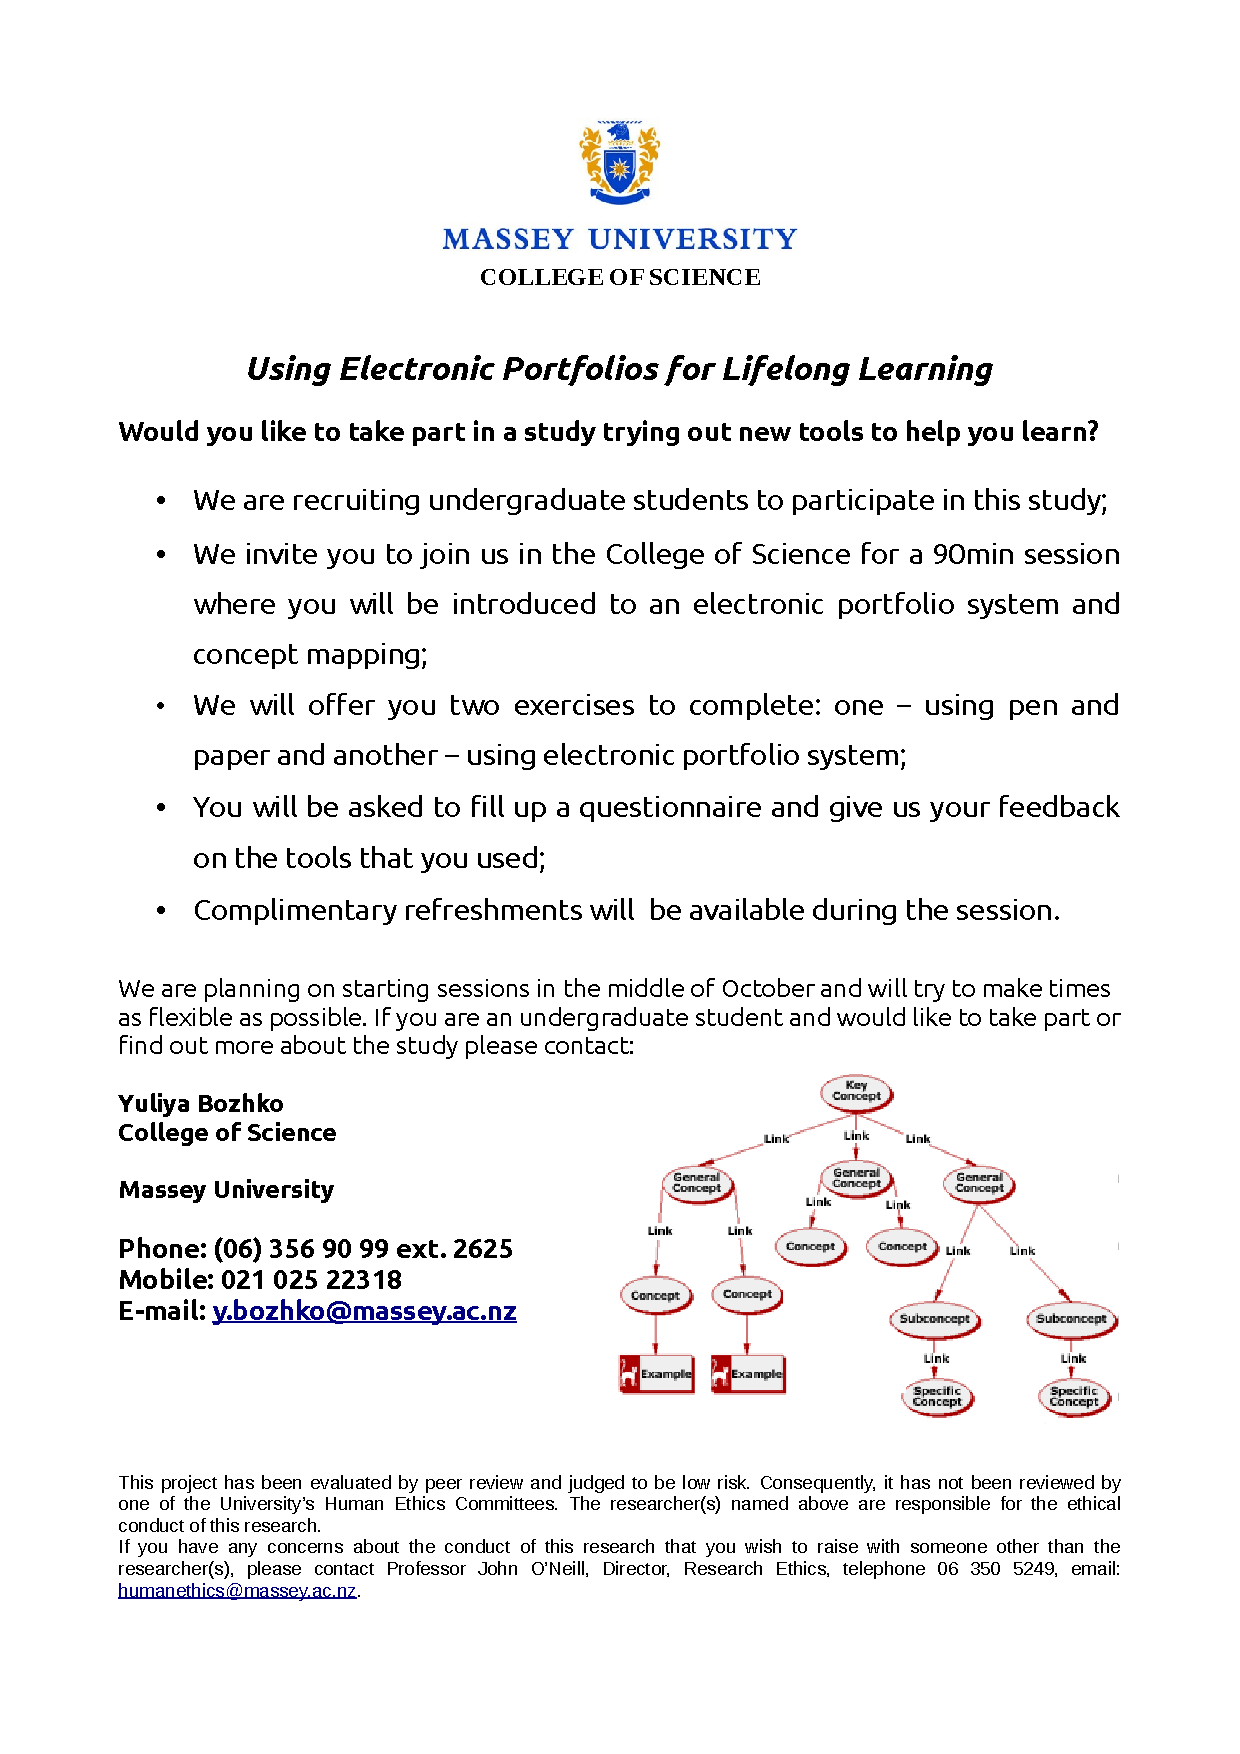
\includepdf[scale=0.7,pages=1,pagecommand=\section{Invitation
Poster},frame]{appendix/Poster.pdf}

\section{Study Protocol}

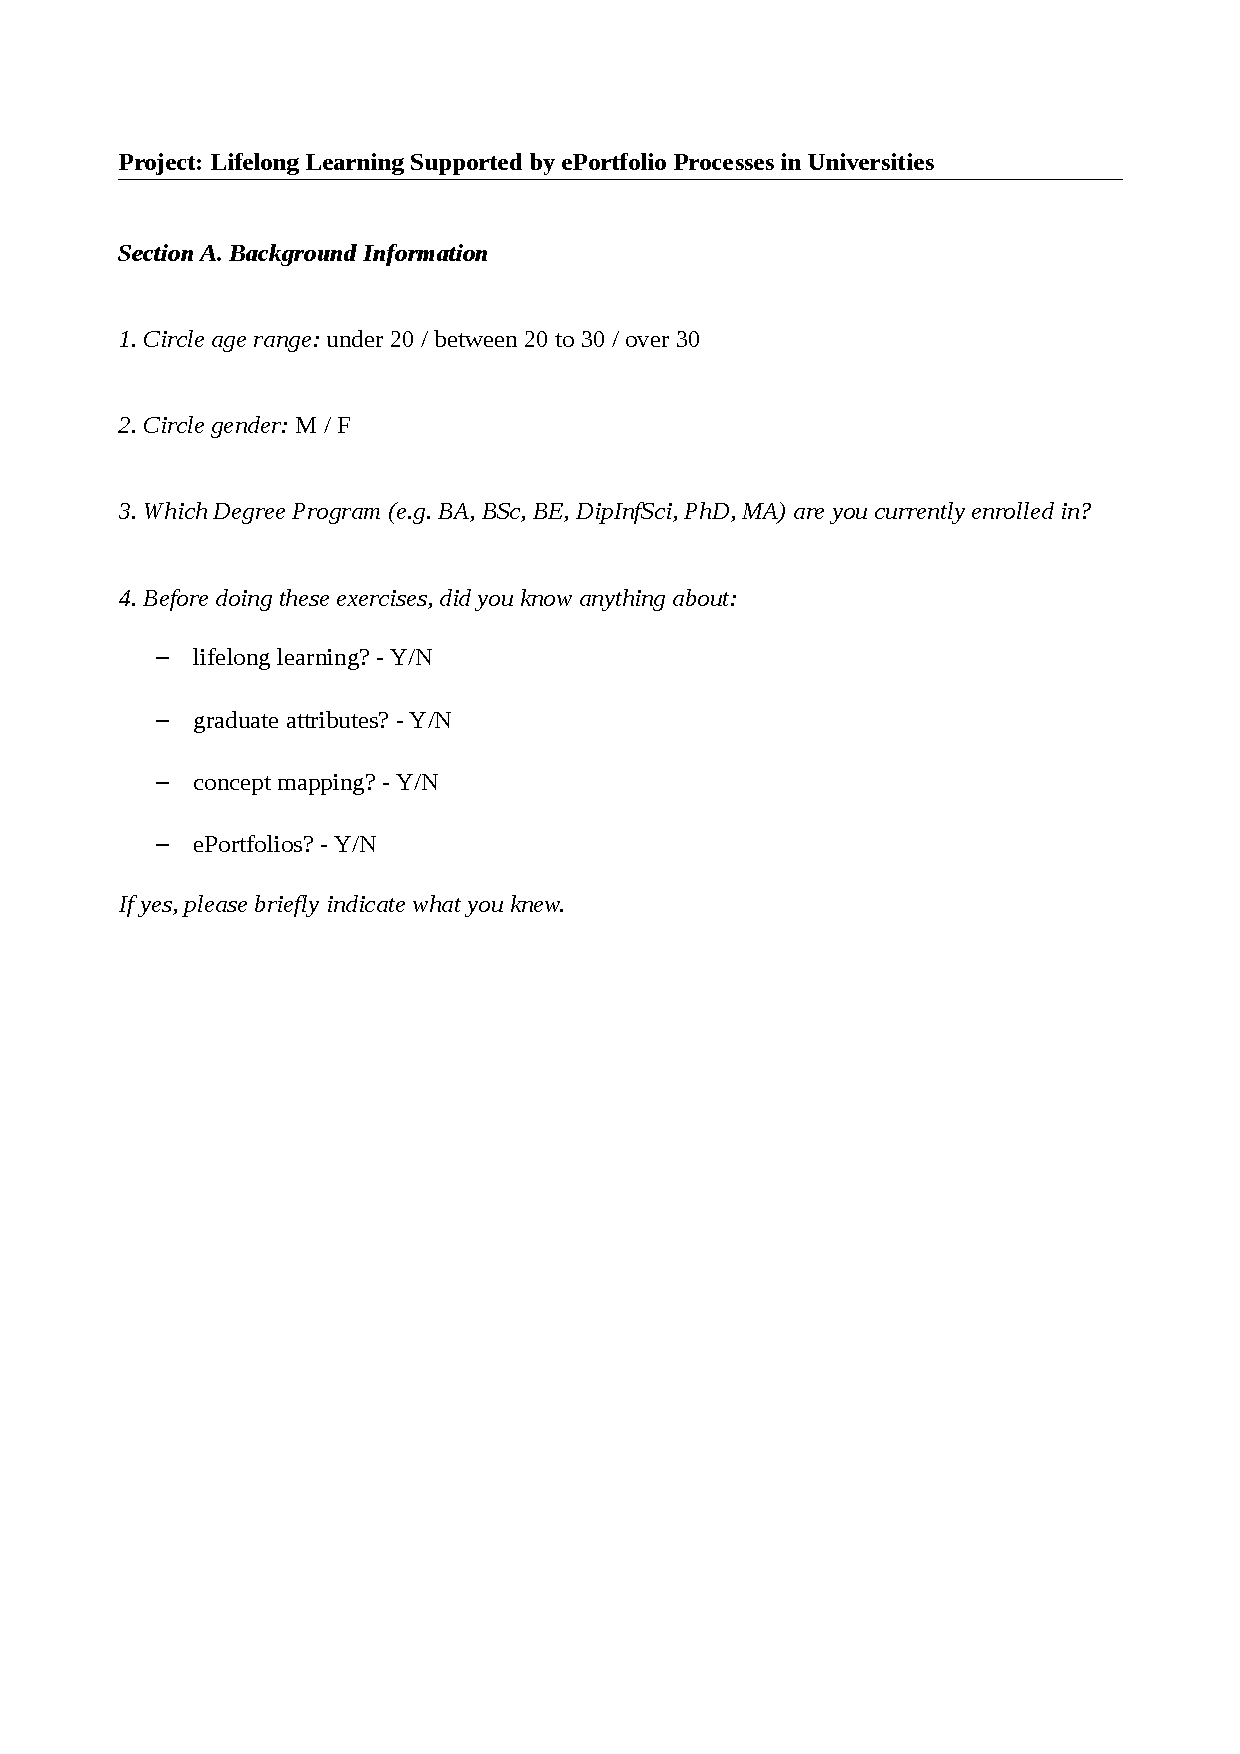
\includepdf[scale=0.7,pages=1,pagecommand=\section{Background and Exit
Questionnaire},frame]{appendix/Exit_u_Q.pdf}
\includepdf[scale=0.7,pages=2,frame]{appendix/Exit_u_Q.pdf}

\section{Concept Map Examples Created by Students}
\label{sec:examples1}

\section{Exit Questionnaire Responses}
\label{sec:responses}
The comments have been combined and reorganised for easier reading of related
ideas.

%=======================================================

\subsection{Potential impact of concept mapping on the development and
understanding of personal learning achievements and graduate attributes.}

\textit{I think that being able to layout concepts in a clear structure like
you can here with definitions and examples would help to cement an understanding
of the significance of what a student has learnt in a specific subject and how
it links to other subjects.}

\textit{It helps to bring in to focus the actual results of studies.
Graphical representation is much easier to recognize and it helps to sort the
ideas. Helps to think about skills over marks.}

\textit{It will help to create clarity in your learning and makes it easier
to learn by breaking things down and being able to see how others are doing this
as well.}

\textit{Would be excellent for creating interactive CV which could be useful
for self-reflection and future employers.}

\textit{It gives a visual understanding of what someone wishes to achieve if the
key concepts are set up before undertaking a course. Over time these concepts can be
modified to reflect on the many experiences gathered. It is a fluid and flexible
system which allows for reflection of anything learnt when people would normally
not realise.}

\textit{Logical system that allows checking of what have been done and what yet
to achieve.} 

\textit{Accountability for own learning.}

\textit{I think concept mapping will really help in these ideas -- I actually
use similar methods in my learning/revision -- just didn't realise what it was
called.}

\textit{A good way of recapping previous work.}

\textit{Simplifies process and makes it much cleaner and more well organized, so
learning achievements and GA are more effective.}

\textit{Makes it easier to follow [own progress], helpful reference that could
be used to supplement written explorations.}

\textit{Great assignment tool -- shows actual development in progress and
thinking.}

\textit{A good way to encourage higher thinking and also communicate thinking
and learning to teachers.}

%=======================================================

\subsection{Most favoured part about concept mapping in the \ep~system}

\textit{User-friendly. Logical, not fragmented like systems I used before.}

\textit{To use artefacts/fragments from our own experience.}

\textit{Presentation -- very informative and clear.}

\textit{So easy to use the concept maps.}

\textit{Opportunity for tagreted reflection.}

\textit{Gets the thinking process going.}

\textit{Being able to add link and examples to the concept maps.}

\textit{It shows learning in a logical, visual way. This is better than writing
an essay with footnotes as we have been doing.}

\textit{Clear flow effect.}

\textit{Easy to use and information is projected in an attractive way.}

\textit{Allows you to make connection between different graduate attributes.}

\textit{Most of all I like that it allows me to can see bigger picture of
my learning and developement.}

\textit{The fact that examples can be fragmented and inserted into a particular
subconcept and the date added to remind or show other people the ``proof'' of the
experience.}

\textit{Good way to keep track of life progress.}

\textit{I like how you can share your thoughts/developments with others and they
can provide you with feedback. I also like how you can branch out as far as you
want to and use bits and pieces of fragments in different places}

\textit{A visual representation makes it easier to think about outcomes (without
actually considering marks).}

\textit{I like that you can separate ideas out into different concepts, each
with definitions and examples and that you can clearly see what would have been
learnt in a specific area and what might extend from this.}

\textit{I liked how easy it is to use. Most software in this area is complicated
and frustrating to use.}

\textit{The way you can show how extracurricular activities count towards your
learning achievements.}

%=======================================================

\subsection{Least favoured part about concept mapping in the \ep~system}

\textit{Fragment part was not very user-friendly}

\textit{That you are restricted to url bookmarks, blogs and uploaded files. For
me, code snippets, twitter and other social networking integration would be
great.}

\textit{Being picky, I would have liked the option to have the concept map going
from top to bottom as well as left to right. Some more explanation about exactly
what each item does and how to add to it and why you would do so would also be
helpful.}

\textit{A little bit confusing at first glance. Easy if you know what you are
doing.}

\textit{Takes a lot of time to construct sometimes.}

\textit{I think, it is rather tricky to navigate through the adding of examples
which certainly can only be done after having a description.}

\textit{Perhaps a little bit difficult starting with a new concept -- just get a
blank page and not sure where to start.}

\textit{Difficult to add examples, but this would come with experience.}

%=======================================================

\subsection{Recommended improvements}

\textit{Would be nice if a box/window popped up with your examples if you hover
the mouse over a definition box.}

\textit{Could be more straightforward when it comes to adding files.}

\textit{Perhaps a step-wise guide to navigating through how to build concept
maps would assist someone who would like to build concept maps on their own.}

\textit{Being able to import files or blogs from other sources (e.g. facebook).}

\textit{Just further explanation about what each part of the system means and
why you would use it. I was able to come away with an understanding because I
was actively trying to understand, but the average user is likely to just want
to be told more explicitly what to do. }

\textit{To create concepts you need to right click. In a web environment this is
rarely used and most users will probably get stuck unless further information is
given. A tutorial on how to setup a basic concept and add files would be useful.}

\textit{Drag and drop in the map would be great as it would add another level
of flexibility.}